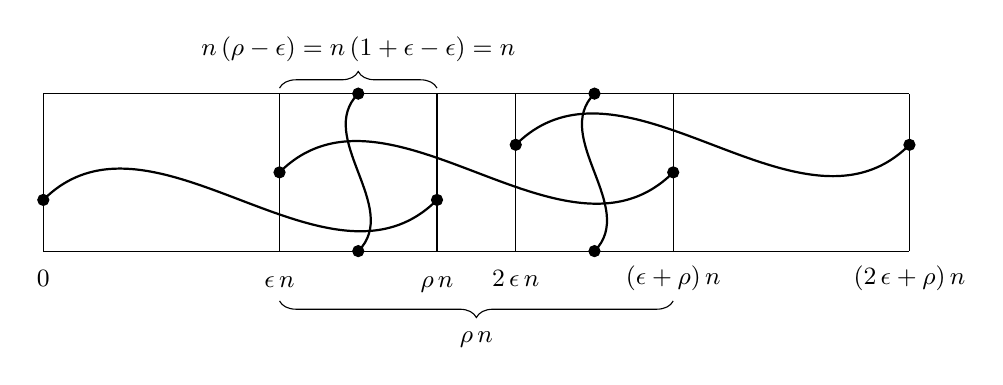
\begin{tikzpicture}[scale = 1]
	\draw[solid, black] (0, 0) -- (5, 0);
	\draw[solid, black] (0, 2) -- (5, 2);
	\draw[solid, black] (0, 0) -- (0, 2);
	\draw[solid, black] (5, 0) -- (5, 2);
	\node[black] at (0, -.35) {{\small $0$}};
	\node[black] at (5, -.42) {{\small $\rho\,n$}};
	
	\draw[solid, black] (3, 0) -- (8, 0);
	\draw[solid, black] (3, 2) -- (8, 2);
	\draw[solid, black] (3, 0) -- (3, 2);
	\draw[solid, black] (8, 0) -- (8, 2);
	\node[black] at (3, -.39) {{\small $\epsilon\,n$}};
	\node[black] at (8, -.35) {{\small $(\epsilon + \rho)\,n$}};
	
	\draw[solid, black] ( 6, 0) -- (11, 0);
	\draw[solid, black] ( 6, 2) -- (11, 2);
	\draw[solid, black] ( 6, 0) -- ( 6, 2);
	\draw[solid, black] (11, 0) -- (11, 2);
	\node[black] at ( 6, -.35) {{\small $2\,\epsilon\,n$}};
	\node[black] at (11, -.35) {{\small $(2\,\epsilon + \rho)\,n$}};
	
	\draw[black, thick] (0, 0.65) to[out = 45, in = -135] ( 5, 0.65);
	\draw[black, thick] (3, 1.0) to[out = 45, in = -135] ( 8, 1.0);
	\draw[black, thick] (6, 1.35) to[out = 45, in = -135] (11, 1.35);
	
	\draw[black, thick] (4, 0) to[out = 45, in = -135] (4, 2);
	\draw[black, thick] (7, 0) to[out = 45, in = -135] (7, 2);
	
	\draw[fill] (0, 0.65) circle (2pt);
	\draw[fill] (5, 0.65) circle (2pt);
	\draw[fill] (3, 1) circle (2pt);
	\draw[fill] (8, 1) circle (2pt);
	\draw[fill] ( 6, 1.35) circle (2pt);
	\draw[fill] (11, 1.35) circle (2pt);
	\draw[fill] (4, 0) circle (2pt);
	\draw[fill] (4, 2) circle (2pt);
	\draw[fill] (7, 0) circle (2pt);
	\draw[fill] (7, 2) circle (2pt);
	
	\draw [decorate, decoration = {brace, amplitude = 6pt}, xshift = 0pt, yshift = 2pt] (3, 2) -- (5, 2) node [black, midway, xshift = 0pt, yshift = 14pt] {\small $n\,(\rho - \epsilon) = n\,(1 + \epsilon - \epsilon) = n$};
	
	\draw [decorate, decoration = {brace, amplitude = 6pt, mirror}, xshift = 0pt, yshift = -18pt] (3, 0) -- (8, 0) node [black, midway, xshift = 0pt, yshift = -14pt] {\small $\rho\,n$};	
\end{tikzpicture}